Table~\ref{tab:main} summarizes the headline numbers for the strict-valid result. The key point is that the reported claim is stable under the saved-candidate threshold sweep and repeated detector recomputation.

\begin{table}[H]
\centering
\begin{tabular}{lr}
\toprule
Quantity & Value \\
\midrule
Stable strict valid ASR & 30.0\% \\
95\% CI & [14.7\%, 49.4\%] \\
Threshold plateau & 0.65--0.80 \\
Full-repeatability mixed flips & 0 \\
Full-repeatability stable candidates & 120/120 \\
\bottomrule
\end{tabular}
\caption{Headline results for the proposed method.}
\label{tab:main}
\end{table}

The observed frontier is more informative than any single point estimate. The highest observed strict-valid result reaches 33.3\% at $K=1$, but the 30.0\% strict result is more robust because it survives both the threshold plateau and 50 repeated detector recomputations.

This distinction matters for interpretation. If one reports only the single best observed point, the result looks slightly higher but less defensible. If one reports the plateau-backed result, the headline number is lower but significantly more robust. We therefore treat 30.0\% as the main strict-valid claim and 33.3\% as the best observed configuration.

\begin{figure}[H]
\centering
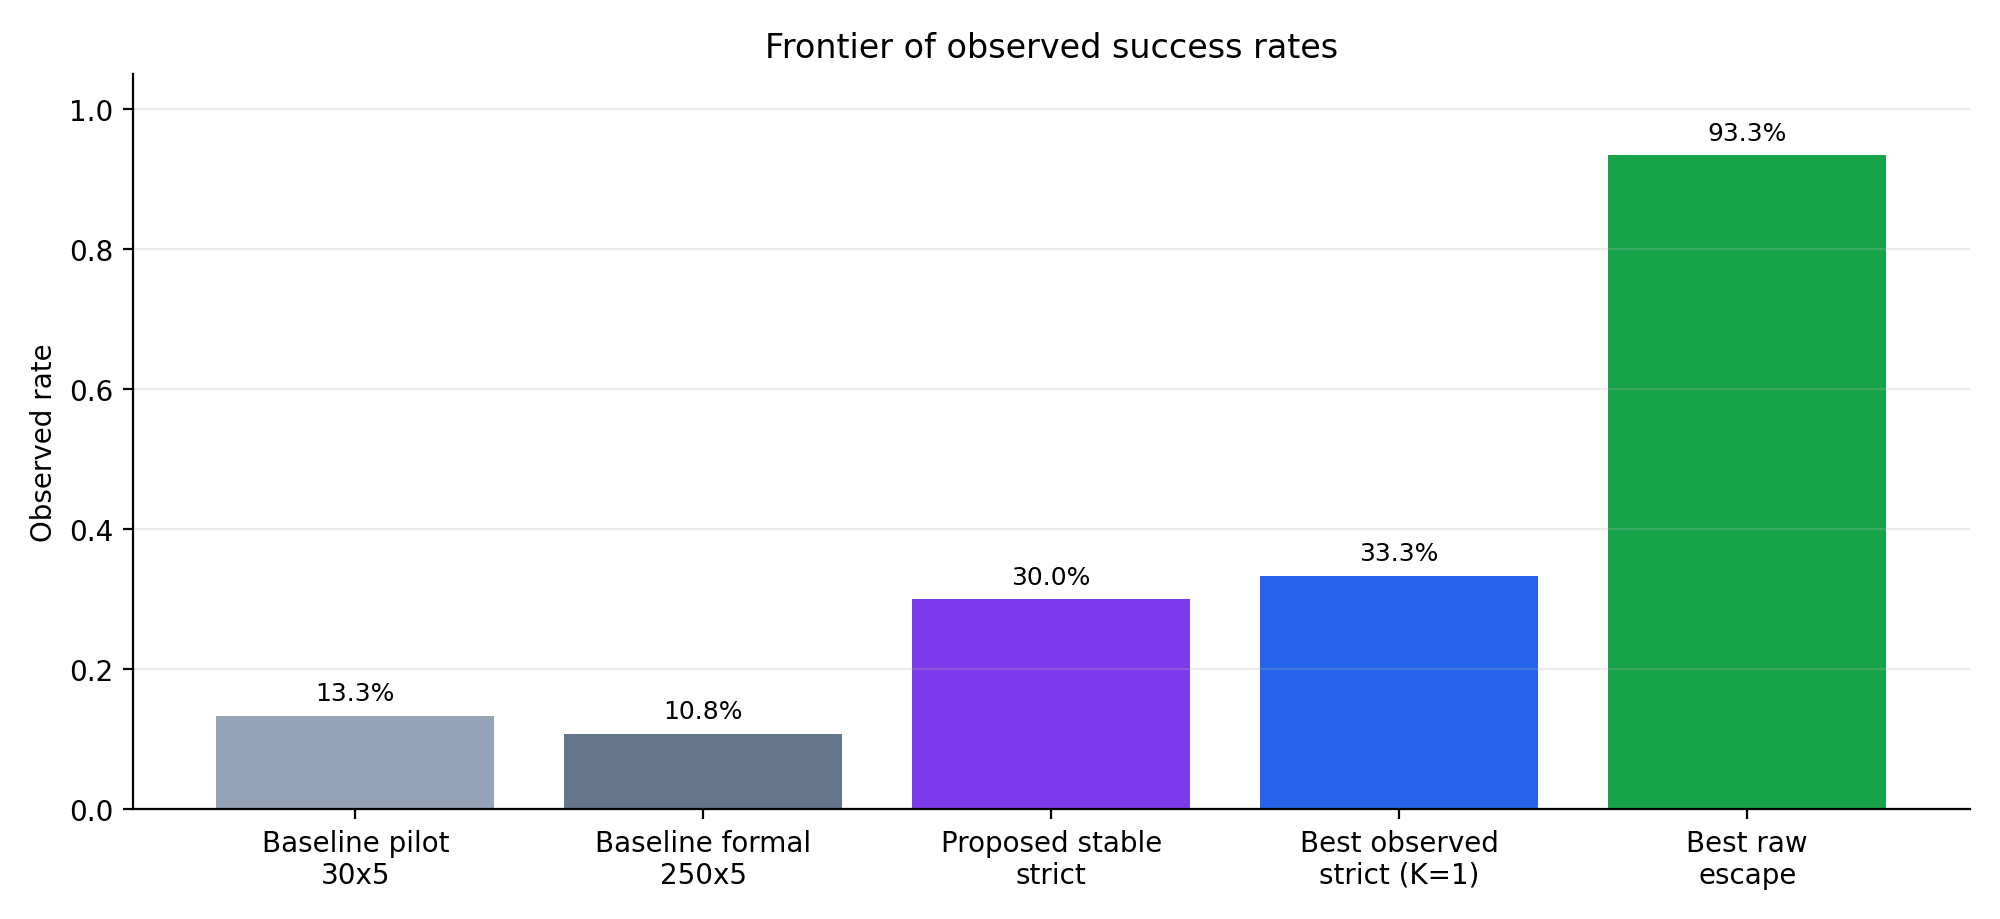
\includegraphics[width=0.92\linewidth]{figures/fig2_frontier.png}
\caption{Observed strict-valid frontier over candidate budget.}
\label{fig:frontier}
\end{figure}

\begin{table}[H]
\centering
\begin{tabular}{lrrrr}
\toprule
Baseline & n & Mean z & Escape rate & AUROC \\
\midrule
Pilot 30x5 & 30 & 3.473 & 13.3\% & 0.998 \\
Formal 250x5 & 250 & 3.439 & 10.8\% & 0.985 \\
\bottomrule
\end{tabular}
\caption{Baseline comparison under the same detector.}
\label{tab:baseline}
\end{table}

Table~\ref{tab:ablation} summarizes the prompt-component ablation. Boundary-only rewriting produces the strongest raw detector weakening, but it also carries the clearest quality cost. The full E2 composition occupies the more balanced point in the quality/escape tradeoff.

\begin{table}[H]
\centering
\begin{tabular}{lrrrr}
\toprule
Method & Mean attack z & Mean z drop & Escape rate & AUROC \\
\midrule
Weak paraphrase & 2.526 & 0.645 & 33.3\% & 0.934 \\
No boundary change & 2.268 & 0.903 & 40.0\% & 0.906 \\
Boundary only & 0.166 & 3.005 & 93.3\% & 0.828 \\
Full E2 & 1.208 & 1.963 & 73.3\% & 0.903 \\
\bottomrule
\end{tabular}
\caption{Prompt-component ablation on the 30-prompt subset.}
\label{tab:ablation}
\end{table}

The failure analysis in Figure~4 is consistent with this picture: when the search procedure over-optimizes for detector score, the outputs tend to drift toward repetition, fragmentation, and overly parser-shaped phrasing. The attack surface is therefore real, but the objective is genuinely multi-objective.

\begin{figure}[H]
\centering
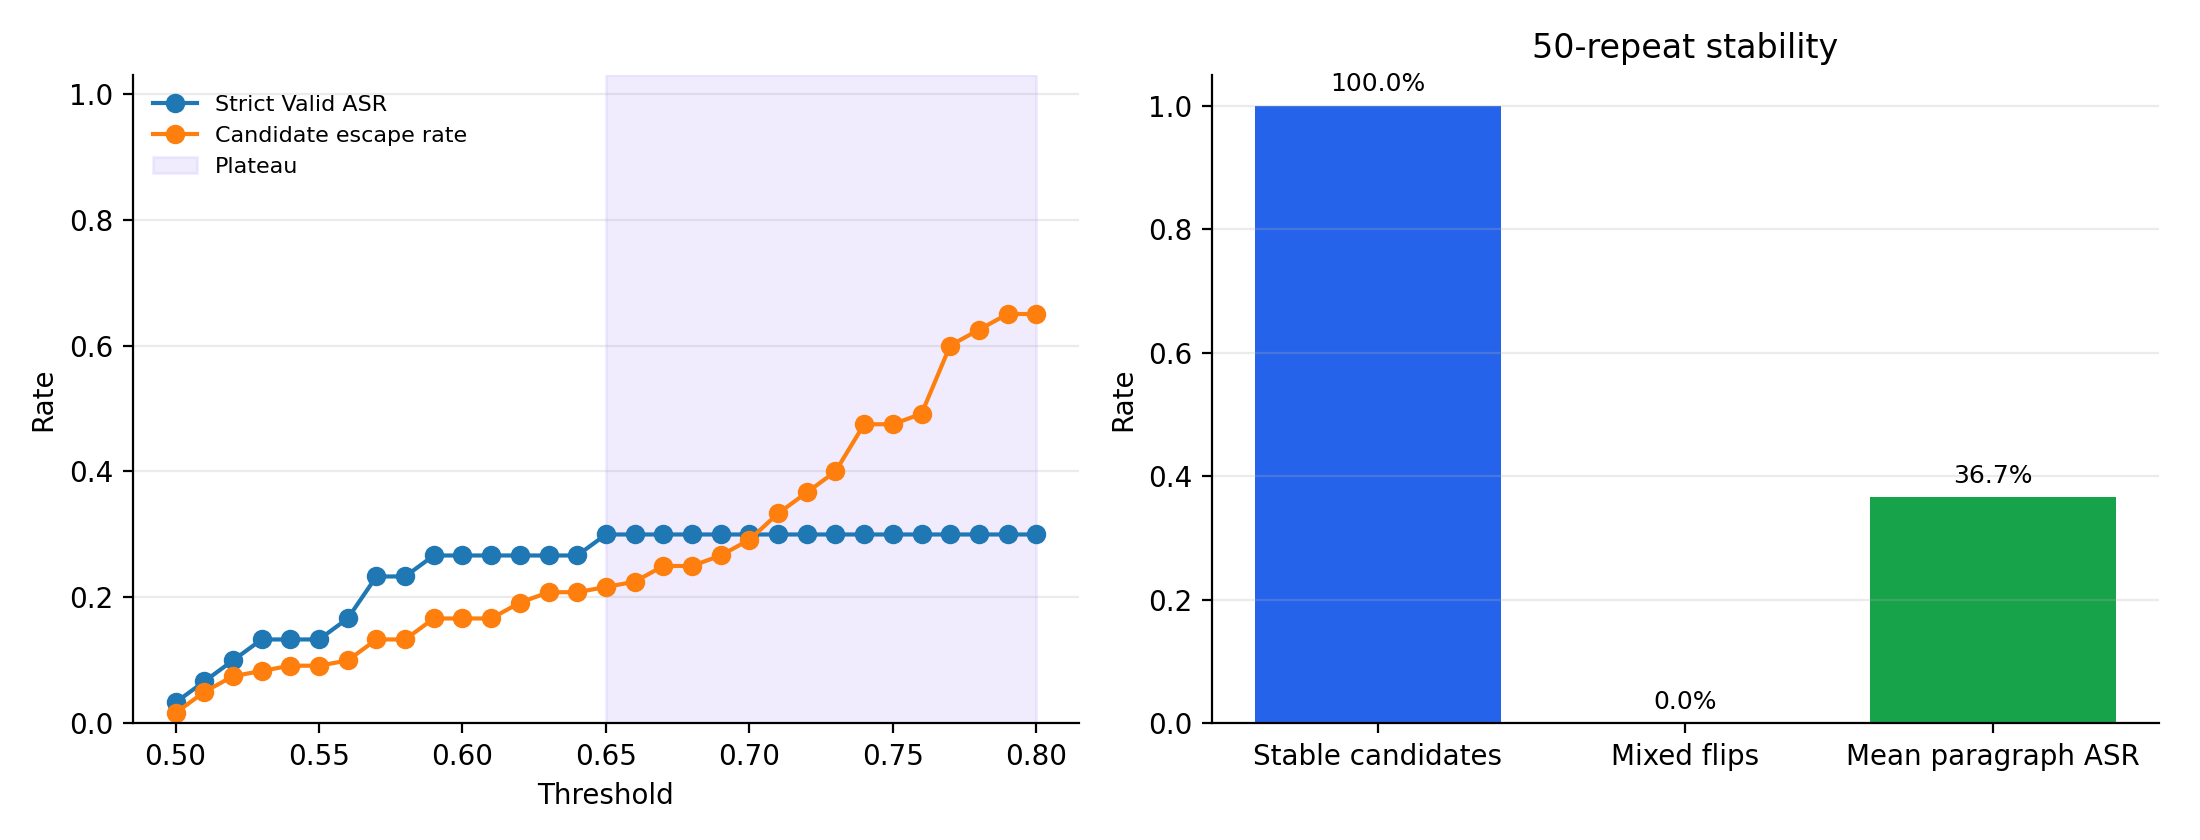
\includegraphics[width=0.92\linewidth]{figures/fig3_robustness.png}
\caption{Threshold sensitivity and repeatability of the strict-valid result.}
\label{fig:robustness}
\end{figure}

\begin{figure}[H]
\centering
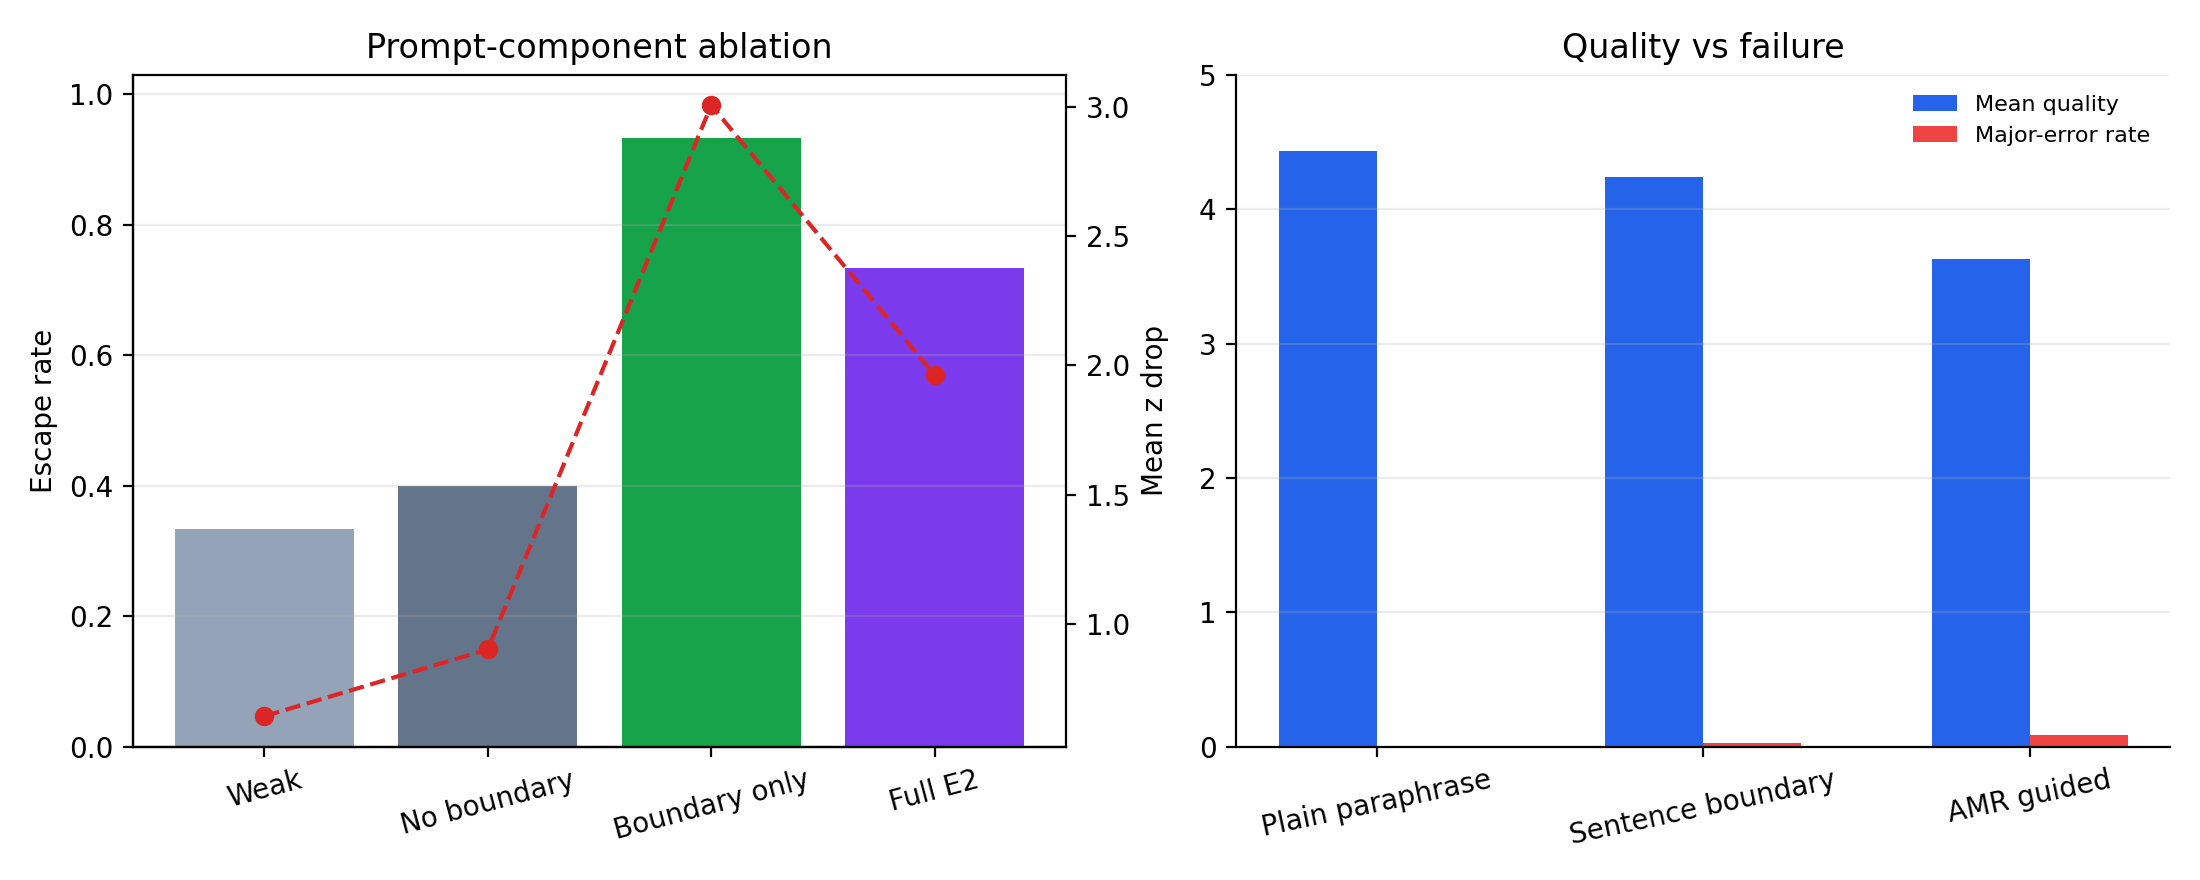
\includegraphics[width=0.92\linewidth]{figures/fig4_ablation_failure.png}
\caption{Ablation and failure-quality tradeoff.}
\label{fig:ablation}
\end{figure}
